\documentclass[11pt]{article}
\usepackage{amsmath}
%\usepackage{extsizes}
\usepackage{amsmath,amssymb}
%\usepackage{omegavn,ocmrvn}
%\usepackage[utf8x]{inputenc}
\usepackage[utf8]{vietnam}

\usepackage{listings}
\lstset{language=Python}          % Set your language (you can change the language for each code-block optionally)


\usepackage{longtable}
\usepackage{answers}
\usepackage{graphicx}
\usepackage{array}
\usepackage{pifont}
\usepackage{picinpar}
\usepackage{enumerate}
\usepackage[top=3.0cm, bottom=3.5cm, left=3.5cm, right=2.5cm] {geometry}
\usepackage{hyperref}


\newtheorem{bt}{Câu}
\newcommand{\RR}{\mathbb R}
\Newassociation{sol}{Solution}{ans}
\newtheorem{ex}{Câu}
\renewcommand{\solutionstyle}[1]{\textbf{ #1}.}
\newcommand{\m}[1]{
	\begin{bmatrix}
		#1
	\end{bmatrix}
}

\begin{document}
% \noindent

\begin{tabular*}
	{\linewidth}{c>{\centering\hspace{0pt}} p{.7\textwidth}}
	Trường ĐHKHTN, ĐHQGHN & {\bf Học Kỳ 2 (2021-2022)}
	\tabularnewline
	K64 TTƯD - Thầy Hà Phi & {\bf Bài Tập Giải Tích Số \\ \today}
	% Exercises on pages 239, 240 Cheney/Kincaid are really nice
	\tabularnewline
	\rule{1in}{1pt}  \small  & \rule{2in}{1pt} %(Due date:)
	\tabularnewline
	%  \tabularnewline
	%  &(Đề thi có 1 trang)
\end{tabular*}




\begin{center}
	{\bf Bài Tập Giải Tích Số. No 6: Các Phương Pháp Lặp (Iterative Methods)}
\end{center}

\begin{bt}
Xét hệ phương trình tuyến tính
%
\begin{equation}
 \m{4 & 1 & 0 & 0 \\ 1 & 5 & 1 & 0 \\ 0 & 1 & 6 & 1 \\ 1 & 0 & 1 & 4} x = \m{1 \\ 7 \\ 16 \\ 14}
\end{equation}
%
a) Viết các công thức lặp Jacobi \& Gauss-Seidel. \\
b) Chuyển các công thức trên về dạng $x^{(i+1)} = K x^{(i)} + k$ trong đó $K$, $k$ là ma trận và vector phù hợp. \\ 
c) Phương pháp lặp sẽ hội tụ khi và chỉ khi $\|K\|<1$. Hãy sử dụng tính chất này để kiểm tra sự hội tụ của các phương pháp Jacobi và Gauss-Seidel trong câu a). \\
d) Nhớ lại phương pháp lặp đơn, ta có $\lambda = \|K\|$. Hãy tính toán $x^{(3)}$, cho trước \linebreak 
$x^{(0)}=\m{0 & 0 & 0 & 0}^T$; và ước lượng sai số hậu nghiệm của $x^{(3)}$. \\
e) Nhớ lại ước lượng tiên nghiệm, hãy tìm $n$ để sai số tuyệt đối của $x^{(n)}$ nhỏ hơn $tol=1e-9$.
\end{bt}

\begin{bt}
\end{bt}
\begin{figure}[!h]
	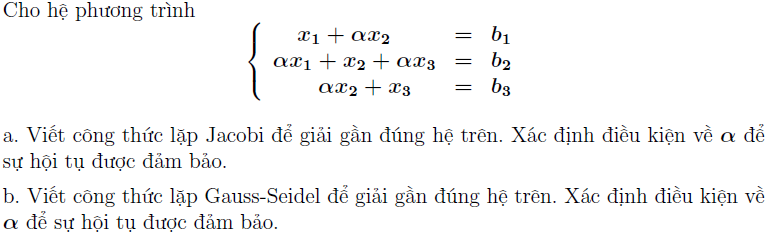
\includegraphics[scale = 0.7]{Figures/5}
\end{figure}


\newpage

\begin{bt}
Các cạnh của tấm hình vuông được giữ ở nhiệt độ như Hình \ref{fig:heatequation}. Giả sử dẫn nhiệt ở trạng thái ổn định, phương trình vi phân điều chỉnh nhiệt độ T trong môi trường là
%
\[
\dfrac{\partial^2 T}{\partial x^2} + \dfrac{\partial^2 T}{\partial y^2} = 0 \ .
\]
%
Nếu phương trình này được tính gần đúng bởi sự khác biệt hữu hạn bằng cách sử dụng lưới được hiển thị, chúng ta thu được các phương trình đại số cho nhiệt độ tại các điểm lưới.	
Hãy giải hệ phương trình thu được bằng các phương pháp Jacobi, Gauss-Seidel, PLU rồi so sánh tốc độ tính toán và sai số.
%
\begin{figure}[h!]
	\centering
	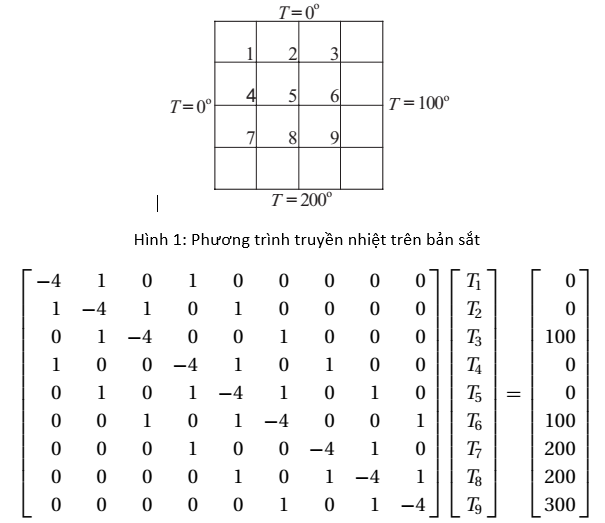
\includegraphics[width=0.7\linewidth]{Figures/heat_equation_3}
	\label{fig:heatequation}
	% \caption{Phương trình truyền nhiệt trên bản sắt}
\end{figure}
%
\end{bt}

\begin{bt}
a) Hãy mở rộng bài tập trên bằng cách thay vì dùng 9 điểm lưới thì dùng 16 điểm lưới. Hệ phương trình thu được là gì? \\
b) Tổng quát hóa bằng $n^2$ điểm, hệ phương trình thu được là gì? \\
c) Giải hệ với $n = 1000$ bằng các phương pháp Jacobi, Gauss-Seidel, PLU rồi so sánh tốc độ tính toán và sai số. Lập trình trong Python để giải quyết bài toán.
\end{bt}

\end{document}

\vspace{1cm}
\noindent{\bf Chú ý:} {\it Cán bộ coi thi không giải thích gì thêm}\\
\Closesolutionfile{ans}
\newpage
\begin{center}
{\LARGE{\bf ĐÁP ÁN}}
\end{center}

\begin{sol}
	\begin{figure}[!h]
		\centering
		\includegraphics[width=0.8\linewidth]{Solution1/Sol4_1.png}
		%\caption{}
		\label{fig:Sol4}
	\end{figure}
	Exercise 7: Convergence order is 3.	
\end{sol}

   
\end{document}



